% Документ принадлежит классу article
%\documentclass[a5paper,8pt]{article} 

% Документ принадлежит классу article, боковые отступы для двустраничной печати.
 \documentclass[twoside,a5paper,8pt]{article}

% нормальный юникод и русский язык
\usepackage{cmap}
\usepackage[T2A]{fontenc}
\usepackage[utf8]{inputenc} 
\usepackage[russian,english]{babel} % Пакет поддержки русского языка
% \usepackage[unicode,dvipdfm]{hyperref}
% \usepackage[pdftex,unicode]{hyperref}

% элементы документа
\usepackage{graphicx}
\usepackage{tabularx}
\usepackage{tabulary}
\usepackage{longtable,tabu}

% показывать структуру страницы в виде рамок: поля, отступы и т.п
%\usepackage{showframe}
%\usepackage{fullpage}
\usepackage[margin=15mm]{geometry}

% ширина картинок с изображением деталей
\newlength{\picwidth}
\setlength{\picwidth}{30mm}

% вертикальный отступ между строками таблицы
\renewcommand{\arraystretch}{5}

 \title{Детали набора Робот Машинка, модель 2.1} % Заглавие документа
 \date{\today} % Дата создания

\begin{document}
  \begin{center}
    \textbf{Инструкция по сборке Робота Машинки}
  \end{center}
  \begin{flushright}
    \emph{модель 2}
  \end{flushright}
   
   
  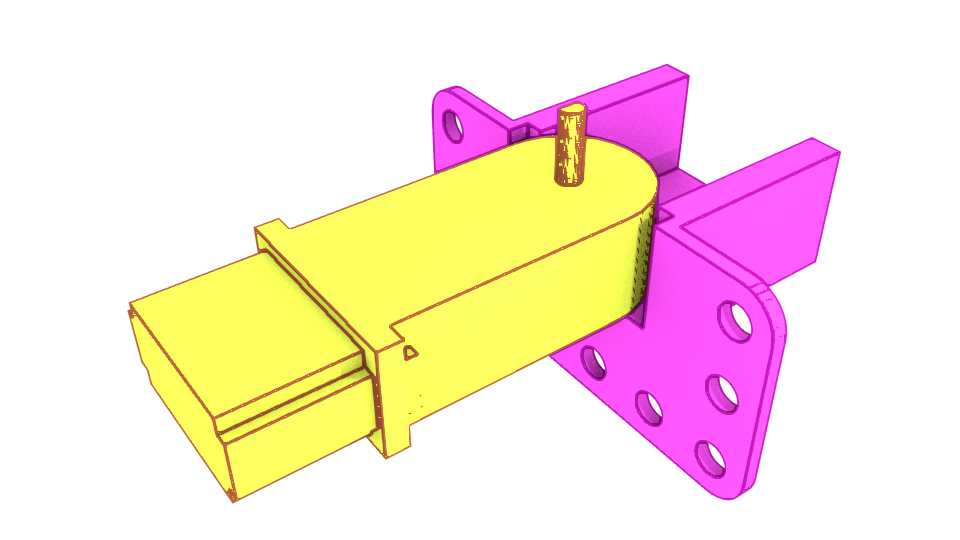
\includegraphics[height=30mm]{blender-render/render-instr/01-motor-block-dev.png}
  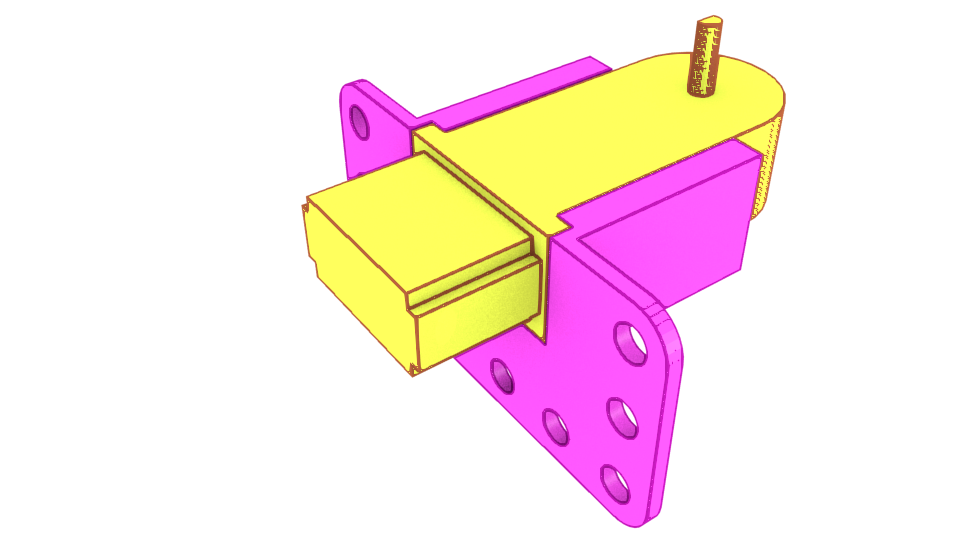
\includegraphics[height=30mm]{blender-render/render-instr/02-motor-block.png} \\
  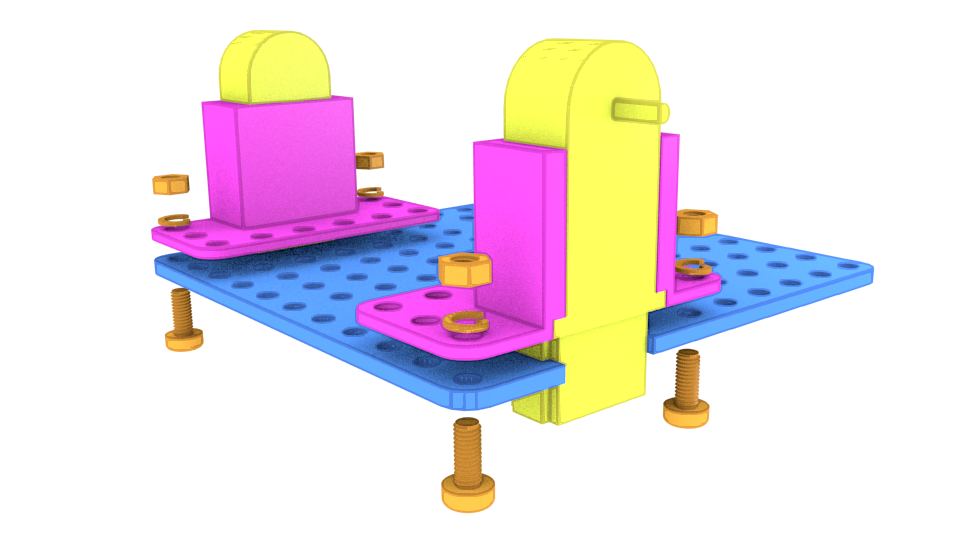
\includegraphics[height=30mm]{blender-render/render-instr/03-top-block1-dev-view2.png}
  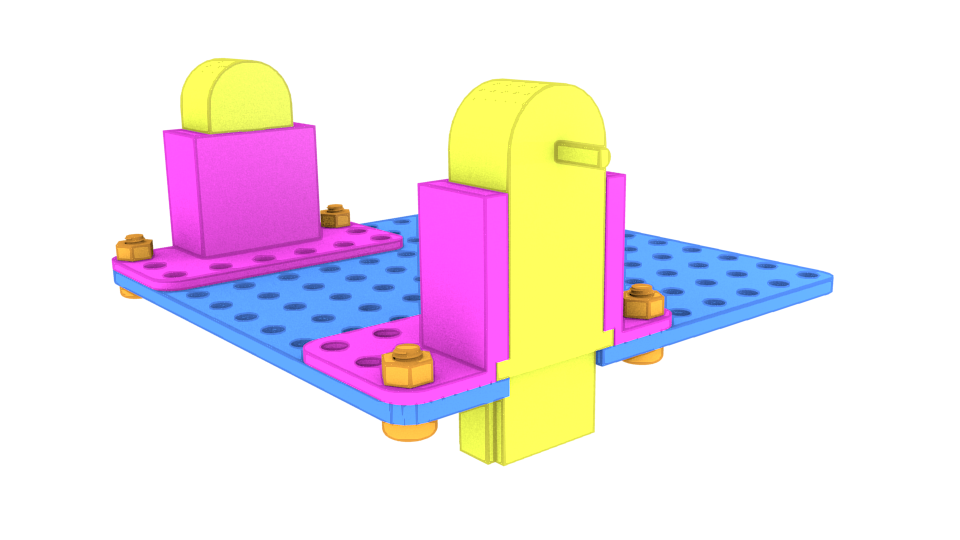
\includegraphics[height=30mm]{blender-render/render-instr/04-top-block1-view2.png} \\
  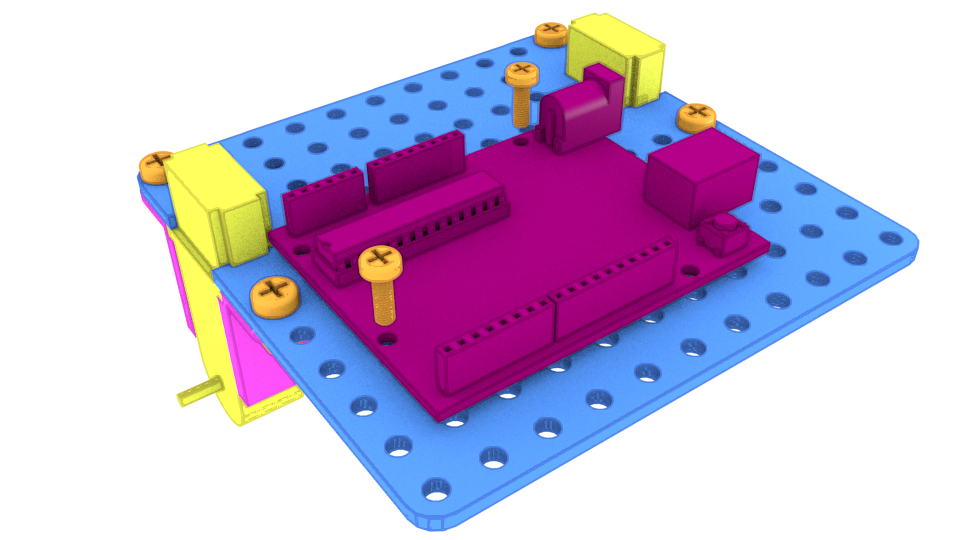
\includegraphics[height=30mm]{blender-render/render-instr/05-top-block2-dev.png}
  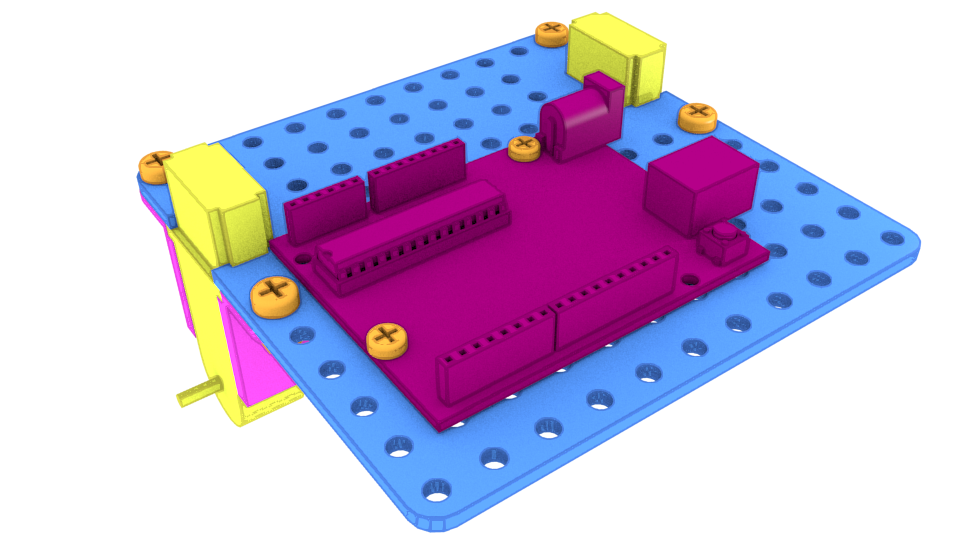
\includegraphics[height=30mm]{blender-render/render-instr/06-top-block2.png} \\
  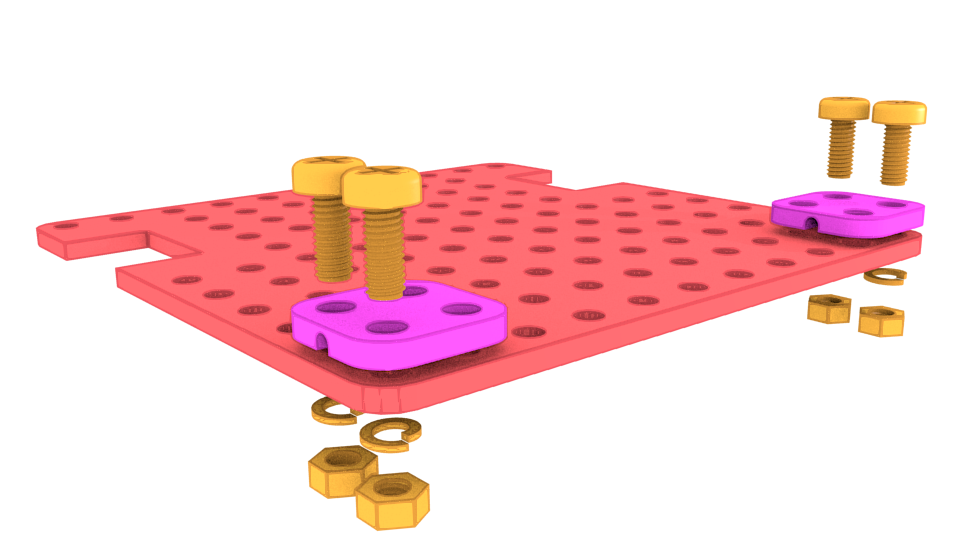
\includegraphics[height=30mm]{blender-render/render-instr/07-bottom-block1-dev.png}
  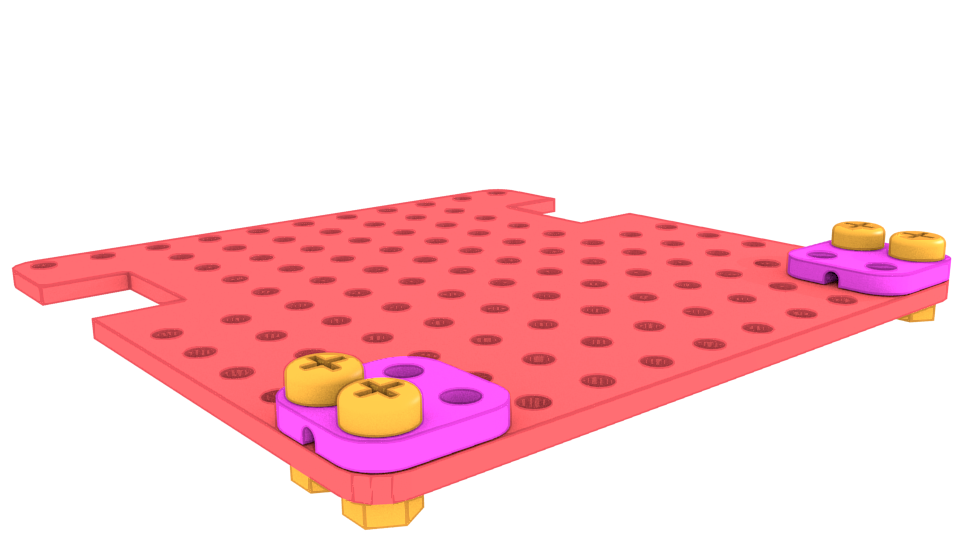
\includegraphics[height=30mm]{blender-render/render-instr/08-bottom-block1.png} \\
  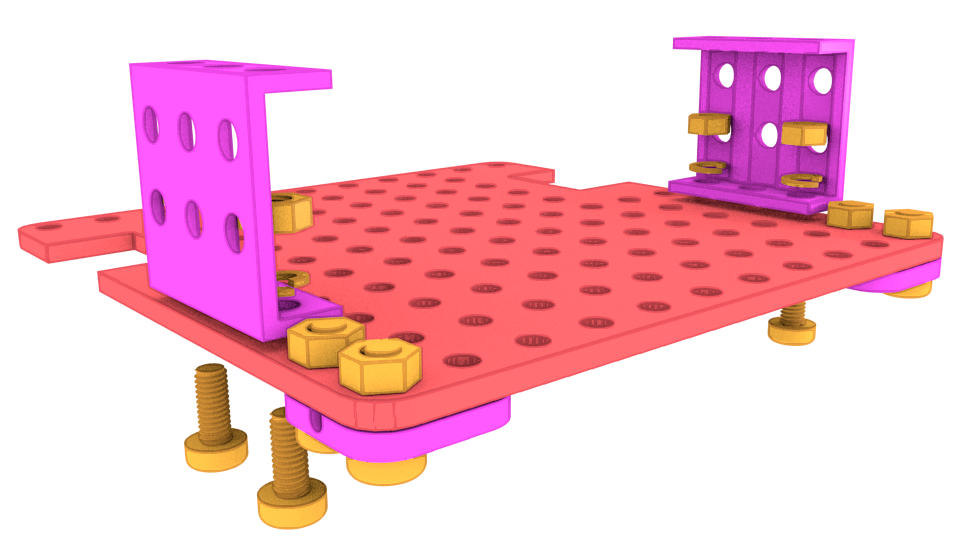
\includegraphics[height=30mm]{blender-render/render-instr/09-bottom-block2-dev.png}
  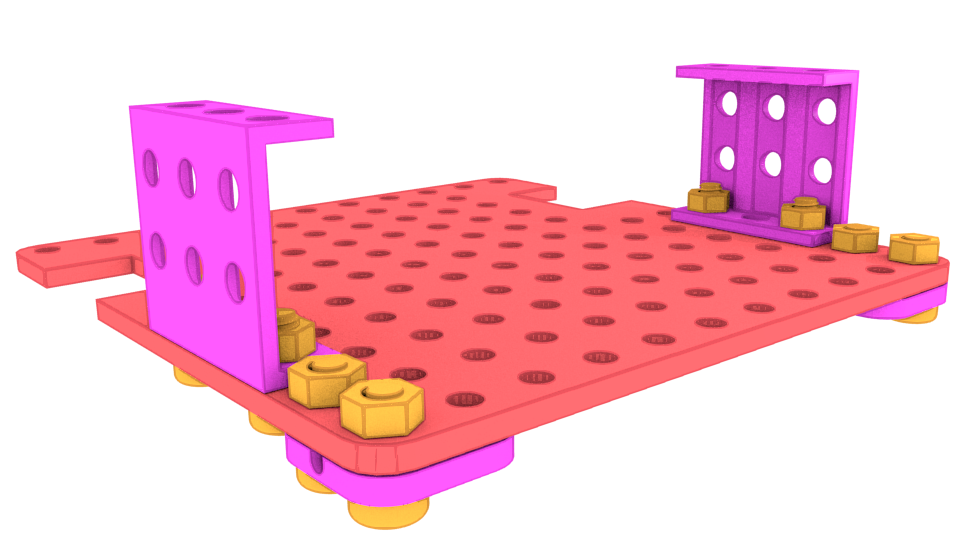
\includegraphics[height=30mm]{blender-render/render-instr/10-bottom-block2.png} \\
  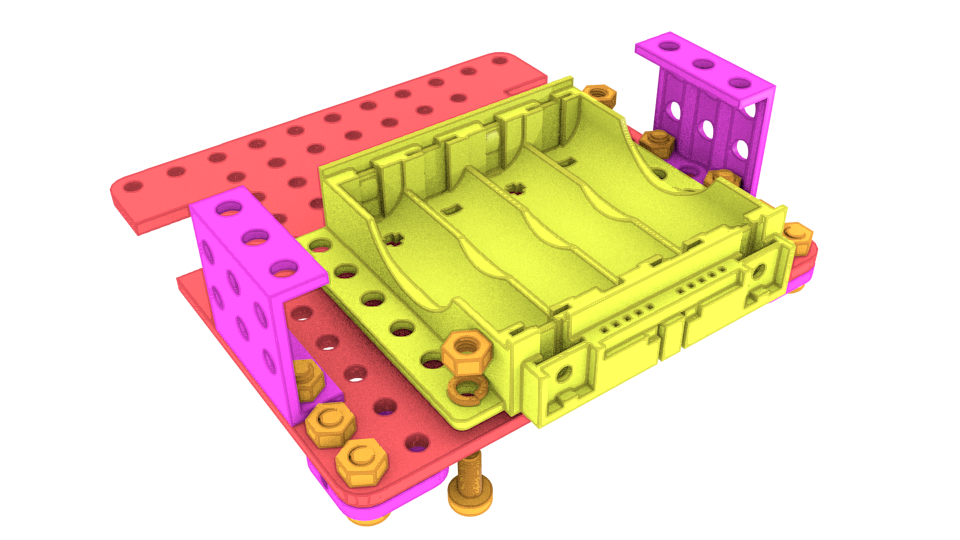
\includegraphics[height=30mm]{blender-render/render-instr/11-bottom-block3-dev.png}
  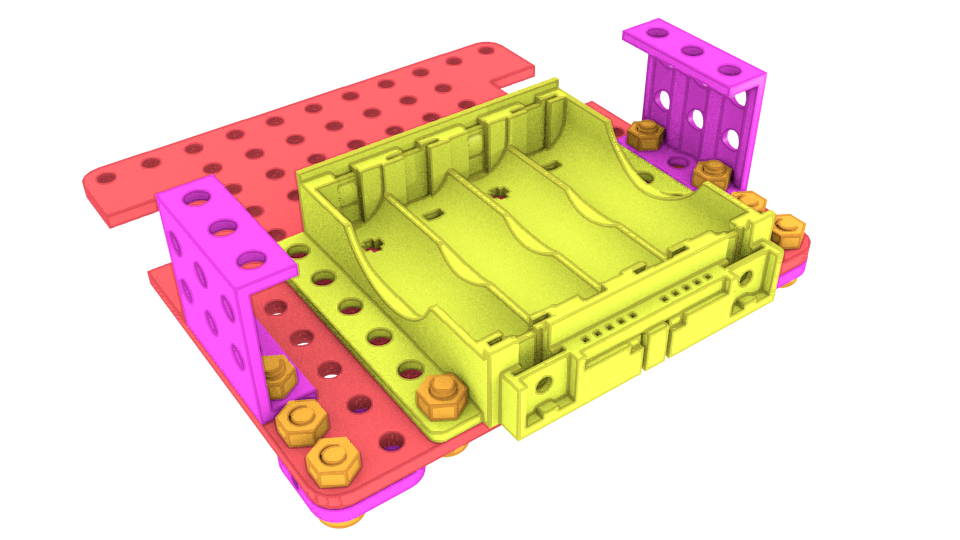
\includegraphics[height=30mm]{blender-render/render-instr/12-bottom-block3.png} \\
  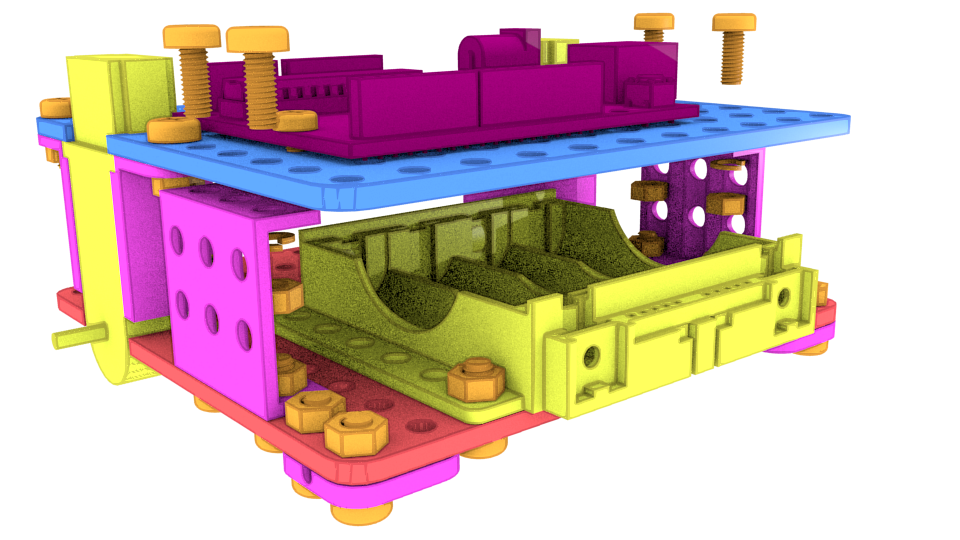
\includegraphics[height=30mm]{blender-render/render-instr/13-frame-block1-dev-view2.png}
  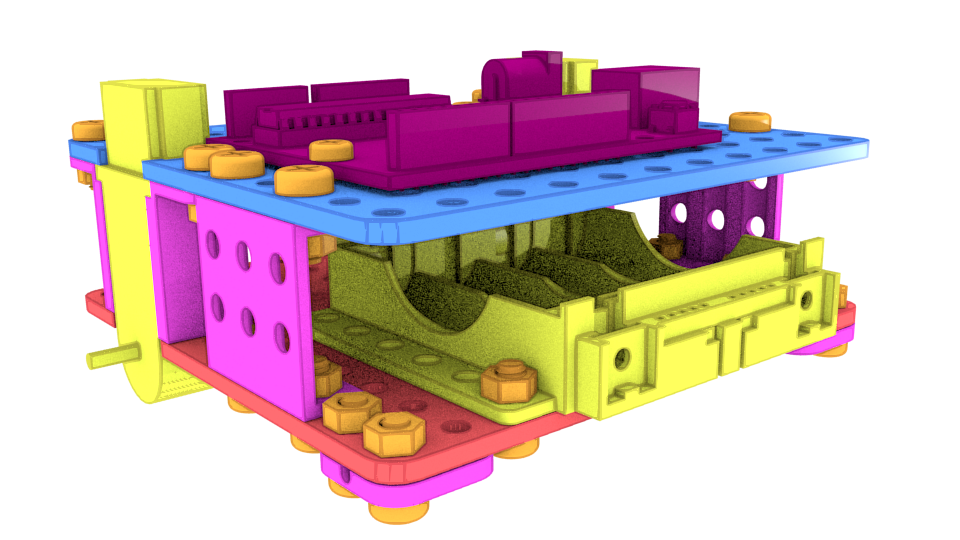
\includegraphics[height=30mm]{blender-render/render-instr/14-frame-block1-view2.png} \\
  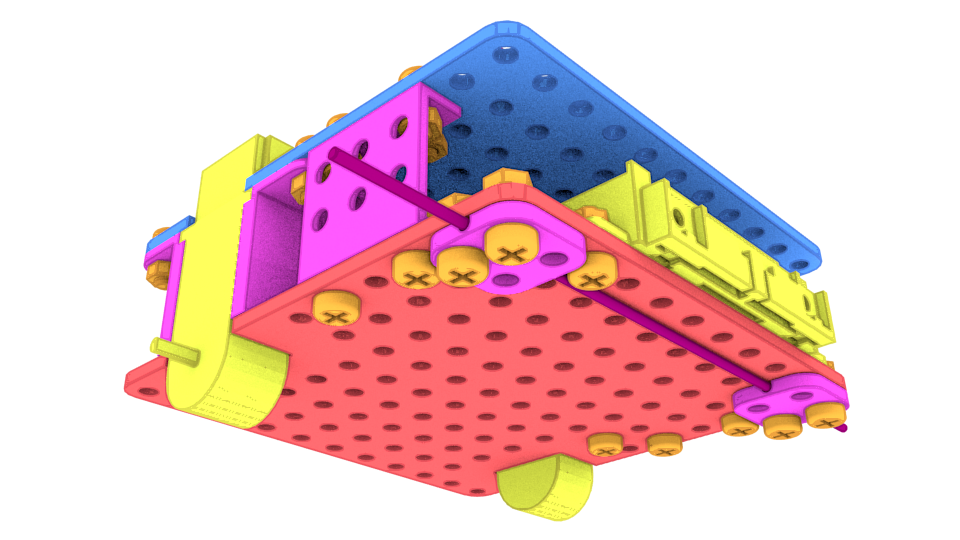
\includegraphics[height=30mm]{blender-render/render-instr/15-frame-block2-dev1-view3.png}
  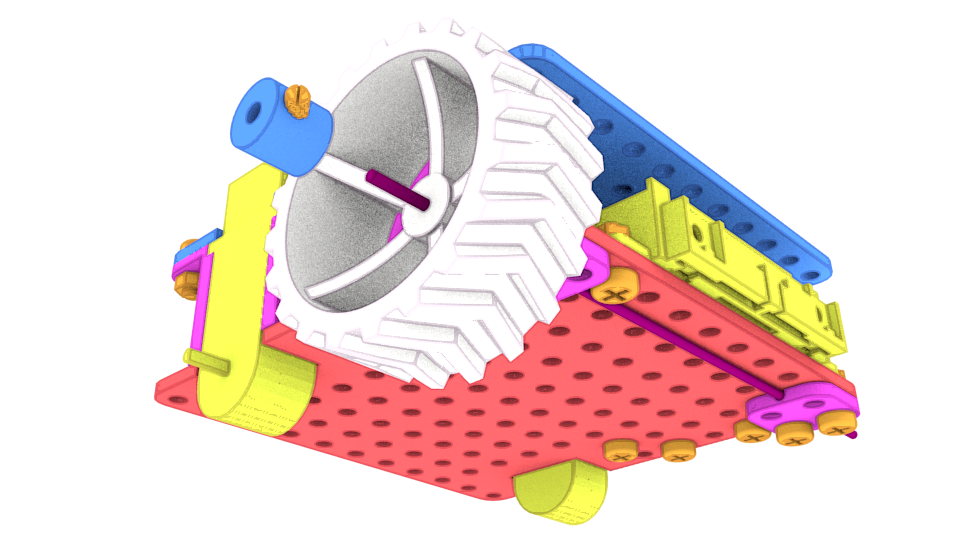
\includegraphics[height=30mm]{blender-render/render-instr/16-frame-block2-dev2-view3.png} \\
  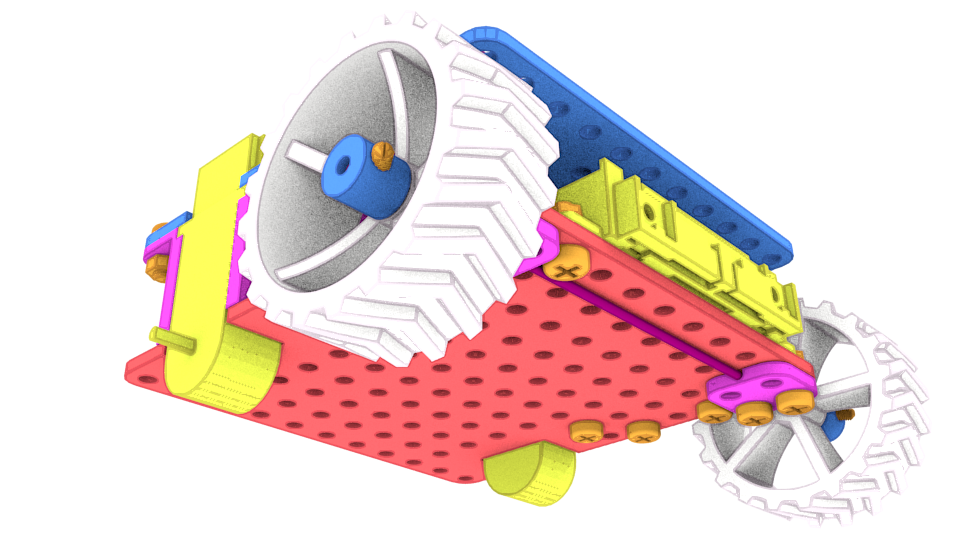
\includegraphics[height=30mm]{blender-render/render-instr/17-frame-block2-view3.png} \\
  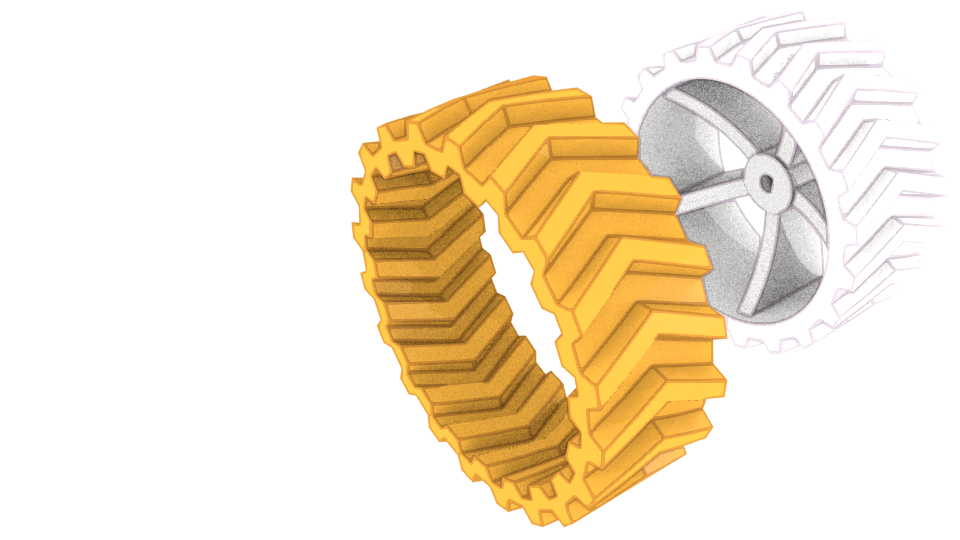
\includegraphics[height=30mm]{blender-render/render-instr/18-wheel-and-tyre-dev.png}
  
\includegraphics[height=30mm]{blender-render/render-instr/19-wheel-and-tyre-view2.png} \\
  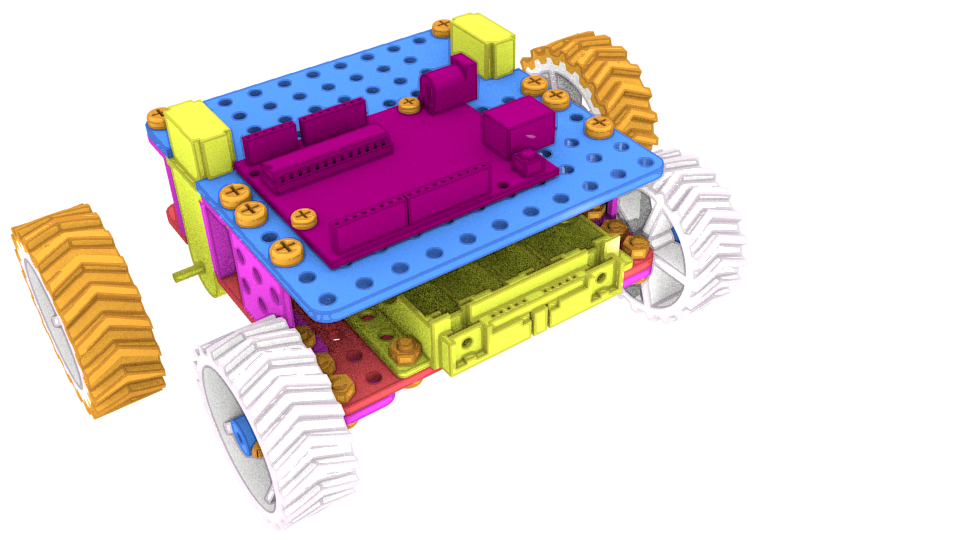
\includegraphics[height=30mm]{blender-render/render-instr/20-frame-block3-dev-view1.png}
  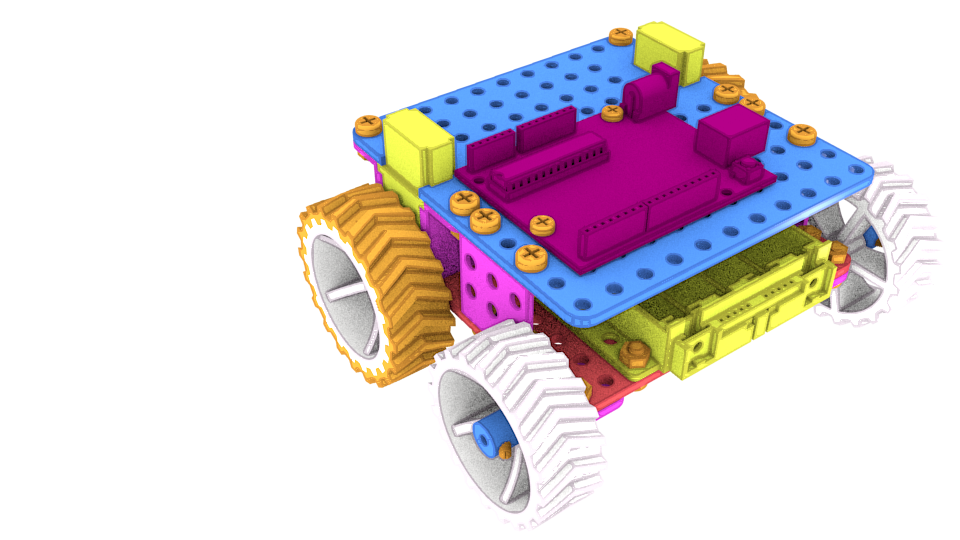
\includegraphics[height=30mm]{blender-render/render-instr/21-frame-block3-view1.png} \\
  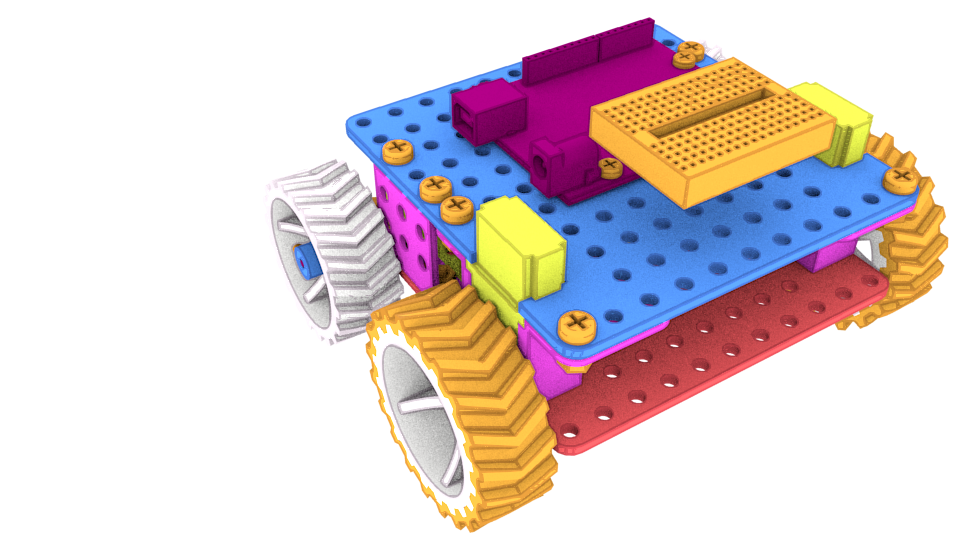
\includegraphics[height=30mm]{blender-render/render-instr/22-frame-block4-dev.png}
  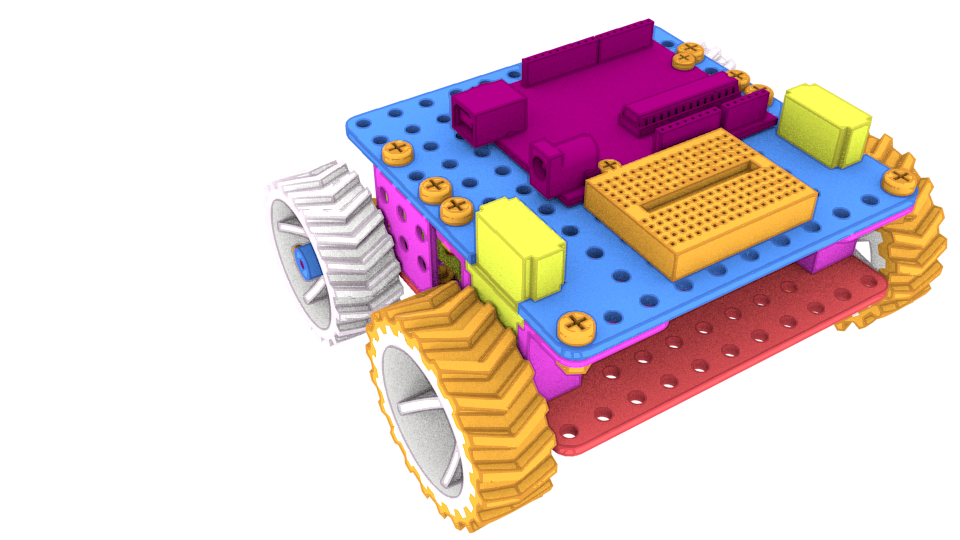
\includegraphics[height=30mm]{blender-render/render-instr/23-frame-block4.png} \\
  

\end{document}
